\documentclass[11pt]{article}
\usepackage{geometry} % see geometry.pdf on how to lay out the page. There's lots.
\usepackage{hyperref}
\usepackage{graphicx}
\usepackage{gensymb}
\usepackage[affil-it]{authblk}
\usepackage[toc,page]{appendix}
\usepackage{pifont}
\usepackage{amsmath}
\usepackage{amssymb}
\usepackage{relsize}
\usepackage{draftwatermark}
\usepackage[mathscr]{eucal}
\usepackage{amsmath, amssymb, graphics, setspace}

\newcommand{\mathsym}[1]{{}}
\newcommand{\unicode}[1]{{}}

\SetWatermarkText{DRAFT}
\SetWatermarkScale{6}
\SetWatermarkLightness{0.95}

\DeclareMathOperator{\atantwo}{atan2}
\DeclareMathOperator{\sign}{sign}
\DeclareMathOperator{\sense}{sense}

% \geometry{letter} % or letter or a5paper or ... etc
% \geometry{landscape} % rotated page geometry

% See the ``Article customise'' template for come common customisations

\title{Open Recreational Problems: Simplex Chains}
\author{Robert L. Read
  \thanks{read.robert@gmail.com}
}
\affil{Founder, Public Invention, an educational non-profit.}


\date{\today}

%%% BEGIN DOCUMENT
\begin{document}

\maketitle

%% \tableofcontents

\section{Introduction}

The term {\em simplex} means the simplest regular polyhedron. In two dimensions, a simplex is an equilateral triangle.
In three dimensions, a simplex is a regular tetrahedron. In four dimensions, it is just called a simplex.
Presumably one can define a simplex in higher-dimensioned Euclidean spaces as well.

Define a {\em simplex chain} to be a figure of many simplices adjoined face-to-face by a particular rule.
The dimensionality of a face is always one less than the dimensionality of the space. In two dimensions,
a simplex chain is a series of adjoined equilateral triangles joined edge-to-edge.

Let us number the simplices in a chain starting from $0$. Then we can define a simplex chain via a rule
that says which edge of the $n$th simplex to attach the $n+1$th simplex to. In two dimensions, we can
label the edge of the last triangle in simplex chain as {\em anti-clockwise} or {\em clockwise}, or just
{\em left} and {\em right}.

If is clear that the rules ``always go left'' ``always go right'' produced a pretty hexagon, but then starts putting the triangles
right where one already is.

The rule ``go left if $n$ is even, right if it is odd'' is a bit more interesting; it produces a ``ladder'' that goes off
in a straight line. That is, the whole figure is contained with in two parallel lines separated by the height of the triangle.

\begin{figure}
     \centering
     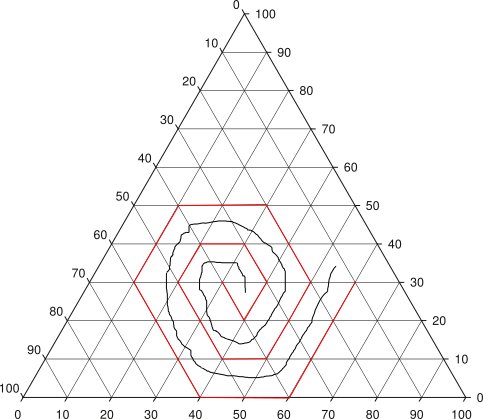
\includegraphics[width=0.65\textwidth]{figures/2DSpaceFilling.png}
     \caption{A Space Filling Spiral}
  \label{fig:equitetrabeam}
\end{figure}


Exercise: There is probably a simplex chain rule which tiles the entire plane with equilateral triangles. Can you define it?

\subsection{The mechanically interesting shapes}

Although simplex chains are interesting in their own right purely theoretic and for recreation,
they are of practical applied value as well.
Mechanical and structural engineers are interested in simplex chains because when constructed out of real, physical
members in the shape of the simplex chain, they may form rigid and structural strong shapes.
For example, many trusses, used to hold up bridges and the roofs of buildings, are in fact simplex chains.

In two dimensions, there are a number of shapes which are interesting not just to mathematicians, but
to engineers and architects. Often, these shapes are made of {\em trusses} which approximate
geometric forms.
In two dimensions the mechanically interesting shapes are:
\begin{itemize}
\item The line
\item The triangle
\item The circle
\item The spiral
\item The sine wave
\end{itemize}

The line is used to make columns and beams. The triangle is the basis of all trusses.
Fractions of circles are arcs used to make bridges. Spirals are used to make clock springs.
The sine wave is similar to the barrel vault and is used to make corrugated roofs and cardboard
and baffles.
Note that the triangle and the circle are closed shapes, the others are not.

General structures in three dimensions made by structural and mechanical engineers are
called {\em space frames}. However, many space frames also follow geometric patterns.
In three dimensions the mechanically interesting shapes are:
\begin{itemize}
\item The beam
\item The triangle
\item The tetrahedron
\item The ring
\item The helix
\item The spiral
\end{itemize}

The beam, the triangle, the ring and the spiral can exist in a narrow space, like inside a wall,
so they are similar to their 2-d analogs, and used for the same purposes.

The helix is used to make staircases and springs and heat exchangers.

Note that the ring and the triangle are a closed shape, the others are not.
The helix does not really exist in two space, although the others do.

The only four-dimensional shape I can conceptualize is that of the
beam: that is, a region close to a line embedded in 4-space.

\section{On ``Open Problems''}

This research effort is focused on real {\em unsolved open problems.}
Usually when we say ``open problem'' in mathematics we mean ``unsolved, probably has a clear objective solution, is valuable,
and is not obvious.''
Open problems you hear about are mostly ones that have been studied a lot and remain unsolved, and are therefore probably difficult problems.
However, in this research-a-thon, many of the open problems are probably easy---they are open and unsolved because nobody has yet
cared to look very closely at them.  However, they are still valuable. Hopefully the problems in this research-a-thon are ``real'', even if they
not as ``hard'' as those professional researchers talk about. 


\section{Relaxations of Regularity}
\subsection{Boundedness}

If we relax the rule that all the lengths of simplex are exactly the same, then it becomes possible to create new figures which are
very close to regular. In particular we can define a simplex chain, or any structure, be {\em $x$-bounded} if the ratio of the longest edge
in the figure to the shortest edge is $x$.

We can then ask questions (in 3D) such as:

What is the smallest number of tetrahedra needed to define an $b+c/b$ torus as a function of $b$ and $c$?

Or:

What is the lowest $x$-boundedness of a figure that defines a torus?

A bound on this number can be given based on my previous work; however, there is almost certainly a better solution that ``twists'' about the torus.

One way to investigate this is simply to place points on the surface of a torus and draw edges between them so as to create an irregular tetrahelix.

\subsection{Rational Regularity}

Define a {\em $k$-regular tetrahelix} to be tetrahelix have at most $k$ distinct edge lengths.
Define a {\em $k$-regular rational tetrahelix} to be a $k$-regular tetrahelix in which all lengths are rational.

We can then ask what is the smallest figure with a hole in each of these dimensions?

Note: There exists a 3-regular rational tetrahelix that is a straight line, or a beam.


\section{Two dimensions}

Two-dimensional shapes are much easier to draw and think about than three-dimensional shapes, but there are still
some interesting open problems.

\begin{itemize}
\item Can we produce more interesting shapes by creating chain rules? (This is largely a recreational problem.)
\item Assuming that all lengths in a regular simplex are of size $1$ and we seek to approximate a circle of radius $r$ with a simplex chain,
  what rule best does that?  What is the best definition of ``best''?
\item If we consider irregular simplices, how do we best approximate a circle?
\item What is the best way to define ``approximating'' a curve with a simplex chain? Is it the sum of the distances of the centroid to the curve?
  Or some notion based on completely covering the curve and not self-colliding?
\item How do we best approximate an Archimedian spiral? A logarithmic spiral? A Fibonacci spiral?
  \item Given an arbitrary curve, how do we best approximate it with a simplex chain, either regular or not?
\end{itemize}

\section{Three dimensions}

The problem of simplex chains in three dimensions is much more interesting. In particular, there is a structure known as the
tetrahelix which is analogous to 2D ladder: it fits inside a cylinder. That is, it is a ``straight'', uncurved stack
of tetrahedra extending infinitely.



\begin{figure}
  \centering
     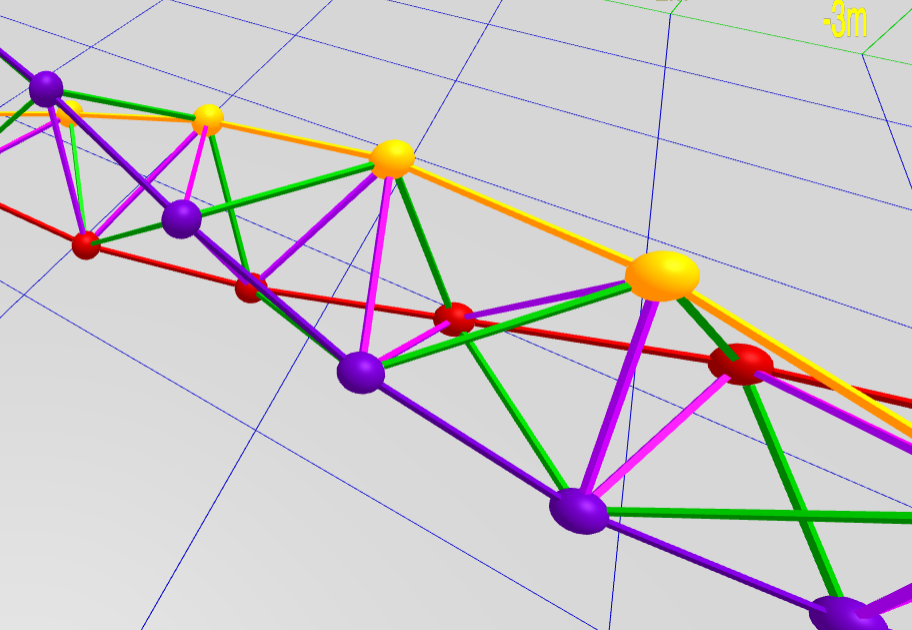
\includegraphics[width=0.45\textwidth]{figures/BCHelixCloseUp.png}
     \caption{BC Helix Close-up (partly along axis)}
  \label{fig:closeup}     
\end{figure}



In order to produce a tetrahelix as a simplex chain, we must have a labeling scheme for the faces of a tetrahedron.
Although symmetric, the first tetrahedron has 4 faces against which we can place the second tetrahelix.
Having placed the second tetrahelix, there are 3 faces against which we can place the third, if we
seek not to collide with the first. These 3 are symmetric; there is no good way to distinguish them,
so in a sense it doesn't matter where we place the third.

But when we come to place the fourth, the figure changes. The three tetrahelices have a clear ``spine''. If we
place the fourth on the face that does not touch the spine, we start to create a shape somewhat like a spindle or a top.
In fact if we carry on this way we can place 6 such tetrahedral, with a 10\% gap remaining. If we carry on, we just keep
going around, creating a solid of revolution.

But what if we place the fourth to the left or right of the spine, and adopt this as a rule? Then we create
clockwise or counterclockwise tetrahelix, respectively, and the we can go on forever, always staying inside a cylinder.
It is curious that the rotation about the center of the cylinder is an irrational fraction of circle, so we will
never come back to precisely the same point.

\begin{itemize}
\item Problem: Can we produce more interesting shapes by adopting more complex rules?
\item Problem: Can we find a rule that fills all space?
\item Problem: If we forbid collisions, can we find a rule that eventually comes near to all points?
\item Problem: What is the maximum fraction of the total volume of 3-Space can we fill (without collisions)?
\item Problem: Can we define a rule that fits inside a torus?
\item Problem: Can we define a rule that follows a helix (that is, that stays close to a helix, as if we took a cylinder and bent it into a helical shape, like a thick wire of
steel coiled into a spring?
\item Problem: Can we define ANY shape that forms a closed loop with no gaps? If not, can we prove that we cannot?
\end{itemize}

Note: We use the term ``equitetrabeam'' to refer to an irregular tetrahelix that has uncurved ``rails'', as in the figure belows:

\begin{figure}
     \centering
     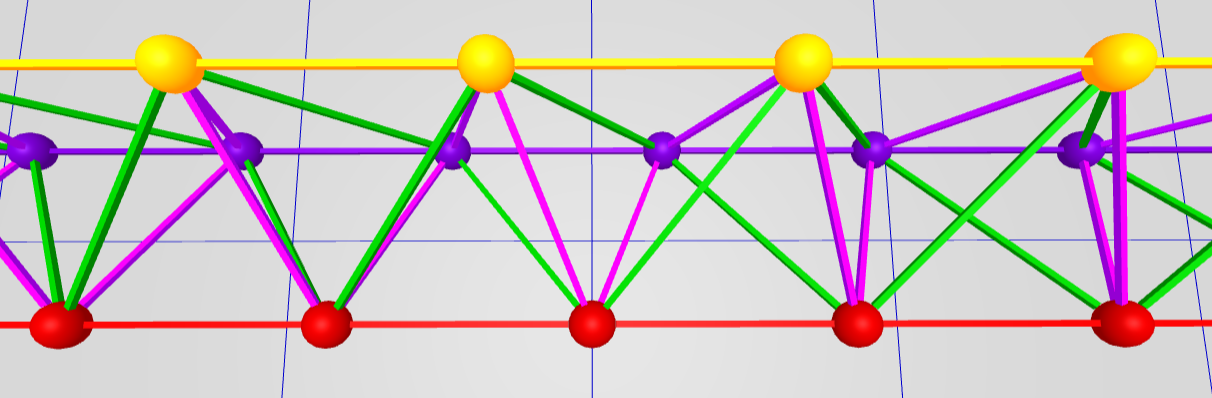
\includegraphics[width=0.65\textwidth]{figures/EquitetrabeamCloseUp.png}
     \caption{Equitetrabeam, an irregular tetrahelix}
  \label{fig:equitetrabeam}
\end{figure}

\begin{itemize}
\item What change length is required to make a finger ring?
\item Clearly Equitetrabeams are stackable, in fact you can make a hexagon of them.
\item Can we make a twisted Equitetrabeam with 3 or 6 columns that is even more efficient?
\item What change length is required to make a  wheel?
\item What is the minimum change length to make a torus?
\item What is the minimum change length of a tetrobot that can touch its toe?
\item What is the densest way to pack a tetrobot into a given volume? (Bounds acceptable)
\item Can we develop easy math for a tetrahelical ``disc touching''?
\item Can we develop math for ``regular variations'' (no kinks)?
\item Can we develop math for ``one kink'' regular variations?
\item Can we make a torus that turns itself inside out, creating circular motion of a point around cross-section of torus?
\item Is there a formula for producing a helix of helices?
\item Is there a way to ``knit'' Tetrahelices into  a slab?
\item Is there a way to ``wind'' tetrahelices into column?
\item Can we do a finite element analysis quickly? What can we discover?
\item Is there a way to build a tensegrity tetrahedron?
\item If there is a tensegrity tetrahedron, how do we mathematically relate to edge lengths?
\item What is the best tetrahelical rail gun?
\item How fast can the tip of a tetrahelix move given a rate of change of member length?
\item Can we improve a software toolkit that let's us play with composing tetrahelices.
\item If we mate tetrahelices face to face, how regular a ``tetrahelical tetrahedron'' can we make?
\item Is it possible to make a perfectly regular structure that has a ``hole''?
\item If it is not possible, what is most regular system that an make a ``hole''?
\end{itemize}

\section{Is there a rule that produces ``straight'' 4D simplex chains?}

If we imagine moving into a four dimensional space, does it make sense to imagine a simplex chain, even though this will have
not solid physical reality as we know it.

The ``face'' of such a figure is in face a 3-dimensional shape, can ``adjoining'' means that two 4D simplices have faces in the same 3D volume.

Possibly we could write a computer program that would allow us to render projections of such figures.
I cannot imagine such shapes, and in a way they become less interesting and less practical than 3D simplex chains.
However, one question seems interesting:

Is there a rule that produces a simplex chain in 4D which would produce a ``straight'' figure?
That is, a figure which always remained within in a fixed distance of a line embedded in 4-space?

Idea: The problem doesn't limit the computational complexity of the chain rule producing the simplex.
However, if we evaluate the simplest rules first, we could write a computer program to simply try a large number
of them. A ``simple'' rule could be considered a function only of the number ``n'' modulo some small number ``m''.

If you consider only simple rules, how does a 4D simplex chain behave? Does it spiral out of control, or remain within
a finite region of space? 


\section{Goals}

For each of the ``mechanically interesting'' shapes, we can ask does there exist a simplex chain,
and if so, what is the smallest,
that matches that shape that has the properties of regularity, $k$-regularity, $k$-rational regularity, and $x$-boundedness. 

\section{Hunting techniques}

In hunting for these open problems, it would be nice to define a toolkit of techniques that we can use.

One technique is to start with a shape you are trying to make, and then place nodes on the surface of the shape,
connecting them to form simplex chains as you go. Then from the shape you have made, consider deriving a simplex chain rule,
if that is possible (it might not be.) In this technique you don't start with a simplex chain rule, but
attempt to find a simplex chain rule.

On the other hand, it may be more elegant to create a simplex chain rule, see what shape is produced,
and then attempt to modify the simplex chain rule to match a shape you are seeking.

\section{Rules of the Mathathon}

\subsection{Rules}

The intention of the Mathathon is to perform all the work in the light and to encourage math
as a social activity.
It is our hope that all members will add their written work to a GitHub repo as quickly
as they can---for example, every 30 minutes or more often would not be unreasonable.
To be eligible for an award on the basis of content, all content must be published in a GitHub repo
whose entire contents are licensed under Create Commons By Attribution(0), or a the
participant must permit their work to be so published in writing.
These repos must remain publicly accessible for one month after the date of the hackathon.

It is preferable to name one file in each repo ``FinalSubmission.pdf'', with the expectation that this
will be the first file read by the judges, and that this file may be included in proceedings, if the
organizers choose to create a proceedings publication.

However, to be considered for an
award all material must be placed in public GitHub repo, or emailed in a pdf before a deadline.
The deadline for email submissions may be early than the deadline for GitHub repo-based submissions.

\subsection{Awards}

Awards at present do not have monetary prizes. If a sponsor provides monetary support, my current intention is to split
the award money evenly between each category below. Participants may receive more than one award.

If sufficient people volunteer, judging will be by a panel of judges.

Awards will be given for:
\begin{itemize}
\item Crowd favorite (to be determined by email vote)
\item Best contribution by someone without a post-baccalaureate degree
\item Best contribution by someone without a college degree
\item Best contribution by someone without a High School degree
\item Best contribution by a Senior Citizen (at least the age of 65)
\item Most creative technique
\item Best contribution by someone not a US Citizen
\item Most worthy of publication
\item Second most worthy of publication
\item Best contribution by a child under 16 (may be accomplished in conjunction with a coach, so long as the child is fully engaged)
\item Best contribution of a new problem statements
\item Most helpful to other participants (not on same team), to be awarded based on written testimonials
\item Second most helpful to other participants (not on same team), to be awarded based on written testimonials
\item Most useful open repo during the mathathon
\item Best mathematical presentation and writing
\item Best code contribution
\item Best contribution of graphic art, figure, or diagram
\end{itemize}

\section{Key Personnel}

Robert L. Read, PhD

\subsection{Potential Key Personnel}

\begin{itemize}
\item Ethan Russo
\item David Jeschke
\end{itemize}


\bibliographystyle{unsrt}
\bibliography{vgt}


\end{document}




\url{https://en.wikipedia.org/wiki/Open_problem}
